\documentclass[compress]{beamer}
\setbeamertemplate{section in toc}[sections numbered]
\usepackage{verbatim}
\usepackage{algorithmic}
\usepackage{mathtools}
\usepackage{xcolor, graphicx}
\newcommand{\x}{{x}}
\newcommand{\y}{{y}}
\newcommand{\w}{{w}}
\newcommand{\W}{{W}}
\renewcommand{\l}{{^l}}
\newcommand{\lplus}{{^{l+1}}}
\newcommand{\lminus}{{^{l-1}}}
\definecolor{Blue}{rgb}{0.3,0.3,0.9}
\newcommand{\textbblue}[1]{{\bf\color{Blue} #1}}
\newcommand{\is}[1]{\setlength{\itemsep}{#1}}
\renewcommand{\Re}{{\mathbb R}}
\DeclareMathOperator*{\argmin}{arg\,min}
\DeclareMathOperator*{\argmax}{arg\,max}


\author{
   		Thomas Hofmann \\[5mm] 
		Institute for Machine Learning \\ ETH Zurich
	} 

\title{
		Advances Deep Learning Models for Cosmology
	}

\date{
		June 10, 2019
	}

\begin{document}

\frame[plain]{\titlepage}

\section{Deep Convolutional Networks}
\frame{\sectionpage}


%%%%%%%%%%%%%%%%%%%%%%%%%%%%%%%%%%%%%%%%
\begin{frame} \frametitle{Deep Neural Networks: Notation}
%%%%%%%%%%%%%%%%%%%%%%%%%%%%%%%%%%%%%%%%
\begin{center}
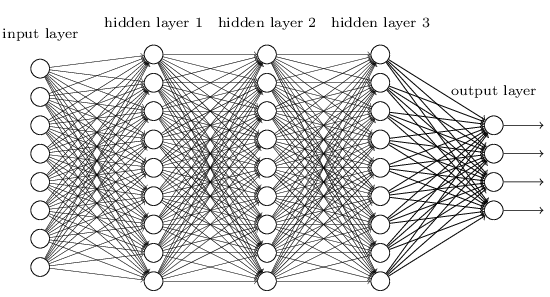
\includegraphics[width=0.52\textwidth]{./figures/OH3gI.png}
\end{center}

Layer-to-layer maps: \textbblue{generalized linear }
\begin{align*}
\x\l = \sigma\l \left( \W\l \, \x\lminus \right), \quad \x\l[i] = \sigma\l\left(\sum_{j} \W\l[i,j]\, x\lminus[j]\right)
\end{align*}
\vspace*{-5mm}
\begin{itemize}
\item layers $l=1,\dots,L$; activations of units $x\l[i] \in \Re$, $i=1,\dots n\l$.\\[2mm]
\item $\sigma\l, \W\l$: fixed activation function / adaptable weight matrix
\end{itemize}
\end{frame}

%%%%%%%%%%%%%%%%%%%%%%%%%%%%%%%%%%%%%%%%
\begin{frame} \frametitle{Convolutional Layers: 1D}
%%%%%%%%%%%%%%%%%%%%%%%%%%%%%%%%%%%%%%%%

Convolutional layer = (discrete) \textbblue{cross-correlation} of (real) signals 
\begin{align*}
y= \w \star \x, \quad   y[t] = \sum_{\Delta t=-m}^m w[\Delta t] \,\, x[t+\Delta t]
\end{align*}
\vspace*{-2mm}
\begin{itemize} \is{2mm}
\item $w[-m\!:\!m]$: filter mask or kernel of width $2m+1$
\item special case of linear model $\y = \W \,\x$, where $\W$ is a bandwidth-limited Toeplitz matrix
\item multiple channels / set of trainable filters
\begin{align*}
\y_r  = \w_r \star \x, \quad r=1,\dots R
\end{align*}
\item parameter sharing ($\equiv$ \textbblue{translation equivariance})
\end{itemize}
\end{frame}

%%%%%%%%%%%%%%%%%%%%%%%%%%%%%%%%%%%%%%%%
\begin{frame} \frametitle{Convolutional Layers: 2D}
%%%%%%%%%%%%%%%%%%%%%%%%%%%%%%%%%%%%%%%%
Simple to generalize to 2D (or 3D, or any dimensionality)
\begin{align*}
y_r= \w_r \star \x, \quad   y_r[s,t] = \sum_{\Delta s} \sum_{\Delta t} w_r[\Delta s,\Delta t] \, \cdot\,x[s+\Delta s, t+\Delta t ] 
\end{align*}
\vspace*{-4mm}
\begin{itemize} \is{2mm}
\item $y_r$: $r$-th feature map
\item stacked feature maps = \textbblue{tensor} ($3$-rd order)
\end{itemize}
\vspace*{4mm}

Composed convolutions in DNNs
\begin{align*}
\tilde \x_\rho\l[s,t] & = \sum_{\Delta s} \sum_{\Delta t} \sum_r w_\rho[\Delta s,\Delta t,r] \, \cdot \, x\lminus[s+\Delta s, t+\Delta t , r]  \\
\x_\rho\l[s,t] & = \sigma\l(\tilde \x_\rho\l[s,t]), \quad \text{(possibly followed by pooling)}
\end{align*}
\end{frame}

%%%%%%%%%%%%%%%%%%%%%%%%%%%%%%%%%%%%%%%%
\begin{frame} \frametitle{AlexNet}
%%%%%%%%%%%%%%%%%%%%%%%%%%%%%%%%%%%%%%%%
{\small \textit{Krizhevsky, Sutskever, Hinton: Imagenet classification with deep convolutional neural networks. NIPS 2012. [40k+cit]}}
\begin{center}
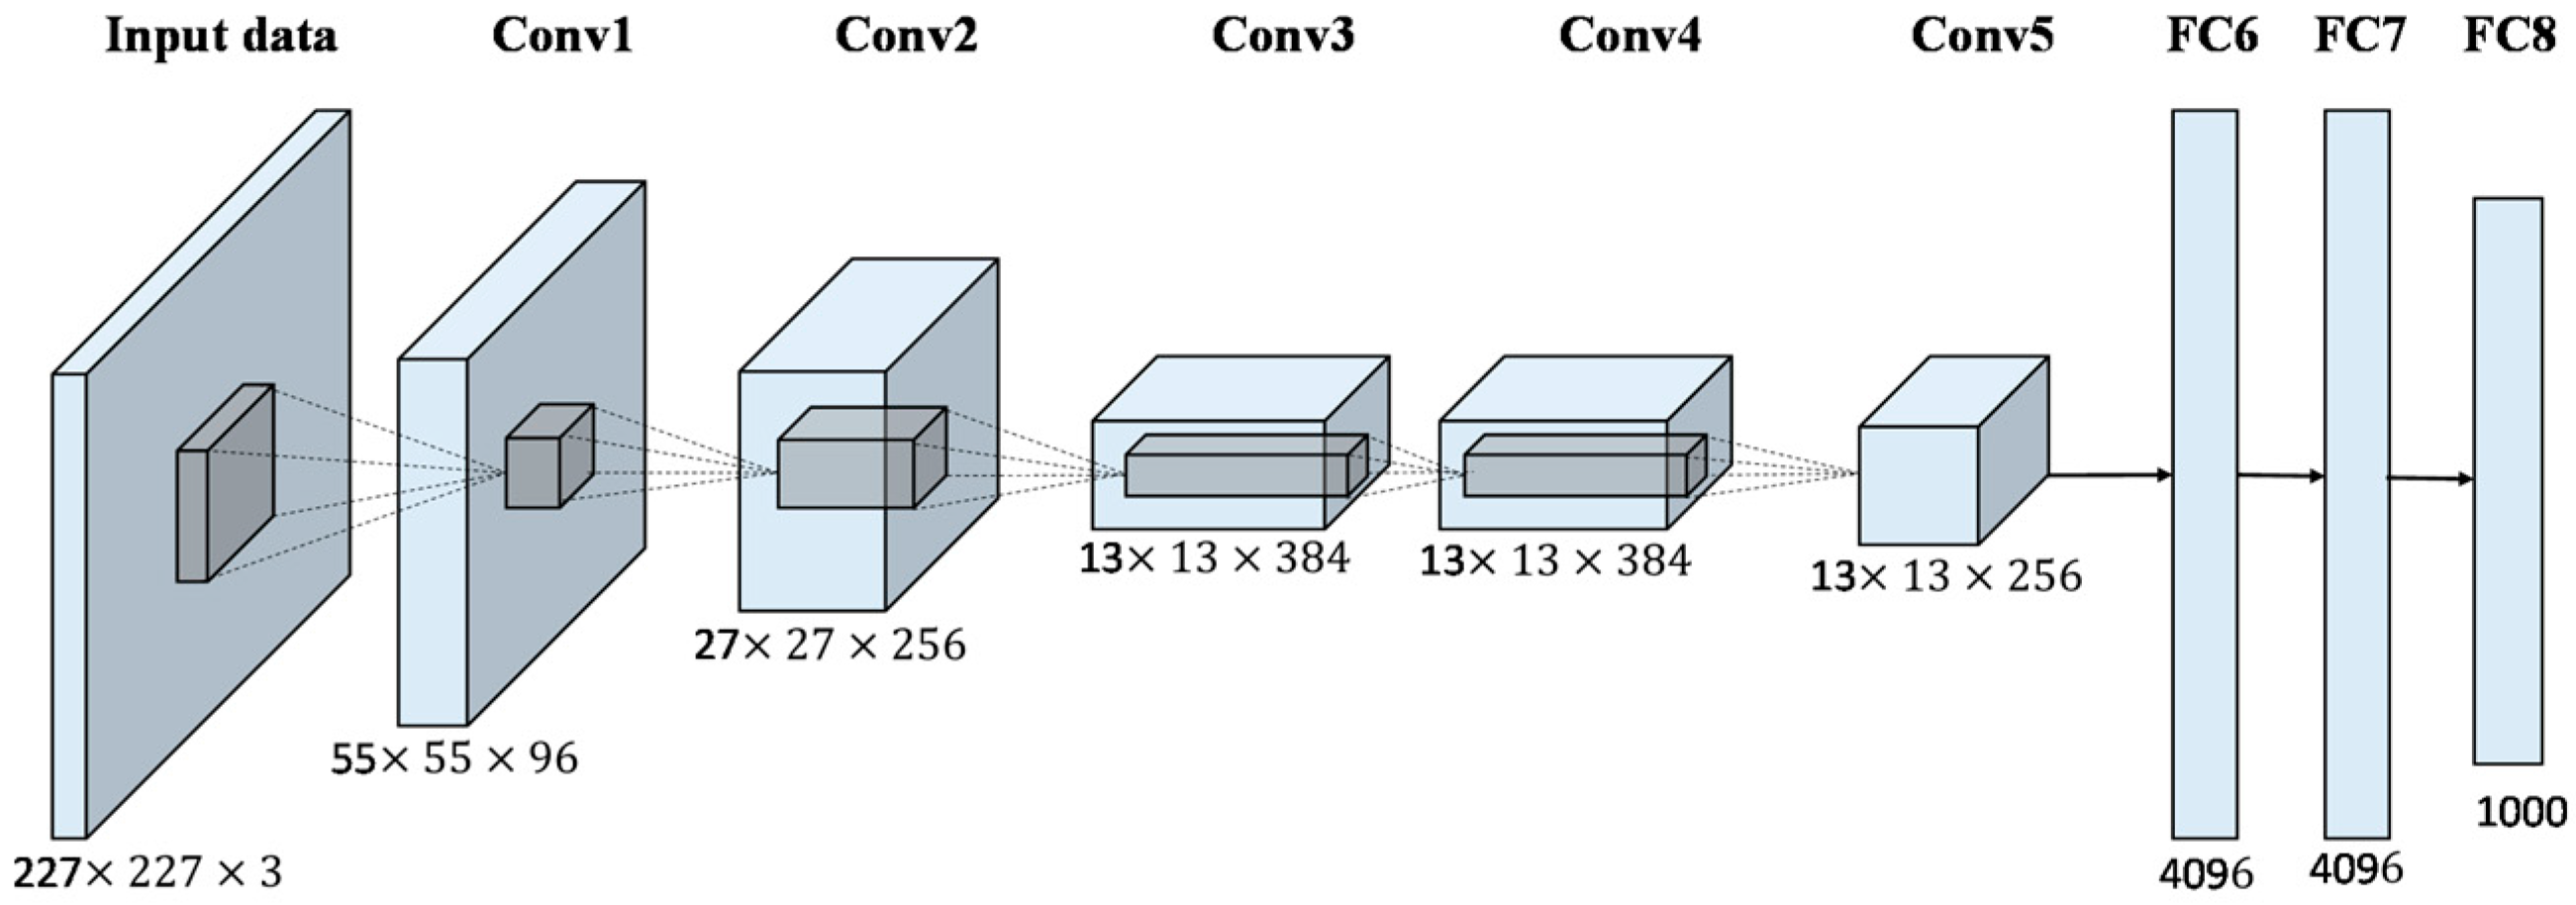
\includegraphics[width=0.7\textwidth]{./figures/alexnet.png}
\end{center}
\begin{itemize} \is{2mm}
\item Typical \textbblue{pyramidal archtecture}: reduce spatial resolution, increase channels with depth
\item Challenge: many channels (width) +large windows +depth
\item Number of parameters
\begin{itemize}\is{1mm}
\item $384$ to $384$ channels with  $3 \times 3$ window: $>1.3$ M
\item $13 \times 13 \times 384$ tensor to $4096$, fully connected: $>265$ M
\end{itemize}
\end{itemize}
\end{frame}

%%%%%%%%%%%%%%%%%%%%%%%%%%%%%%%%%%%%%%%%
\begin{frame} \frametitle{Network within Network}
%%%%%%%%%%%%%%%%%%%%%%%%%%%%%%%%%%%%%%%%
{\small \textit{Lin, Chen, Yan: Network in network. arXiv:1312.4400 (2013) [2.5k+cit]}}
\begin{center}
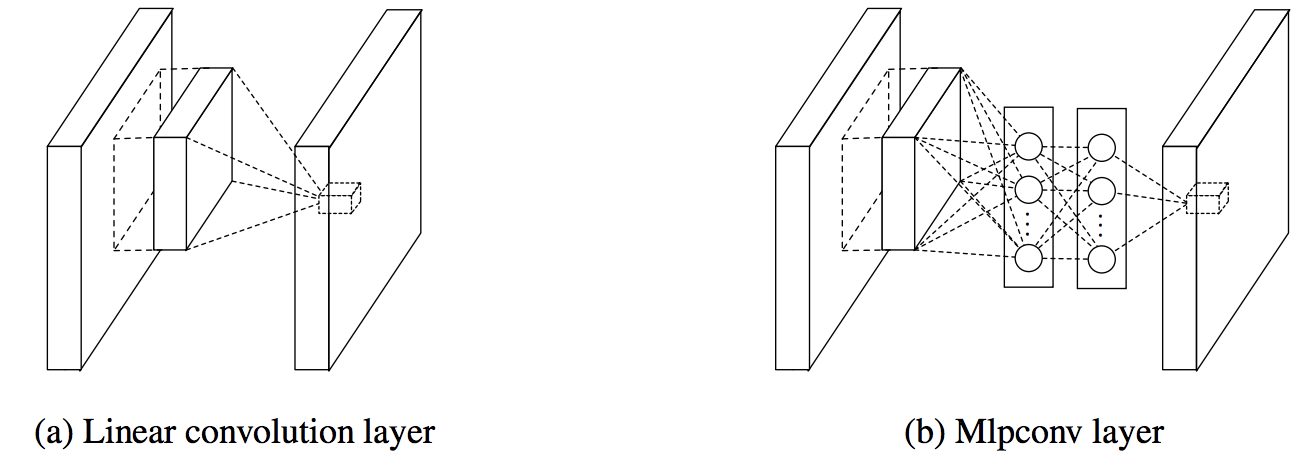
\includegraphics[width=0.8\textwidth]{./figures/netinnet.png}
\end{center}

\begin{itemize} \is{2mm}
\item increase modeling power of generalized linear models by plugging in a multi-layer perceptron (MLP)
\item preserve parameter sharing, yet allows for more complex mappings from tensor patch to vector
\end{itemize}
\end{frame}

%%%%%%%%%%%%%%%%%%%%%%%%%%%%%%%%%%%%%%%%
\begin{frame} \frametitle{Inception Modules and Networks}
%%%%%%%%%%%%%%%%%%%%%%%%%%%%%%%%%%%%%%%%
{\small \textit{Szegedy et al.: Going deeper with convolutions. CVPR 2015 [13.5k+cit]}}

\begin{center}
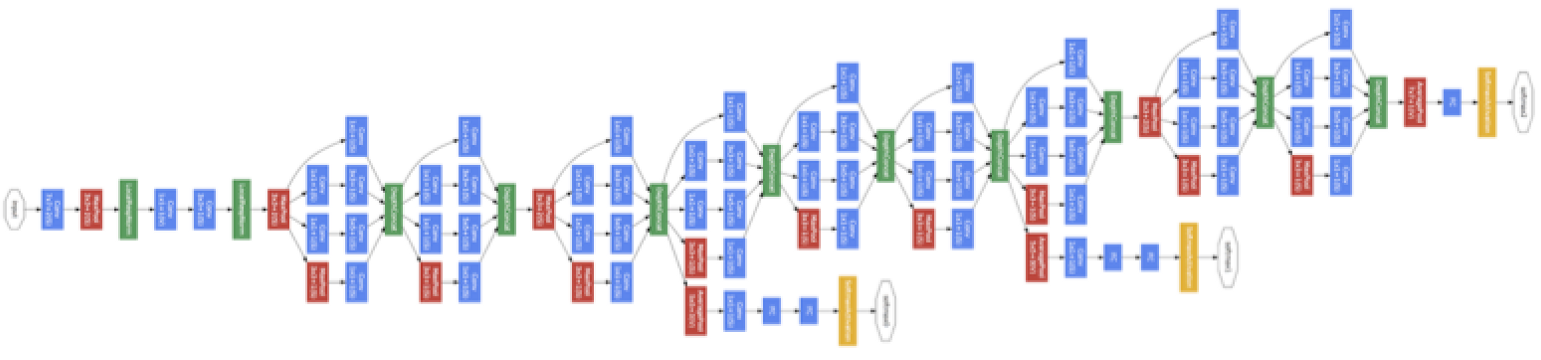
\includegraphics[width=0.8\textwidth]{./figures/inception-network.png}
\end{center}

\begin{columns}
\begin{column}{0.4\textwidth}
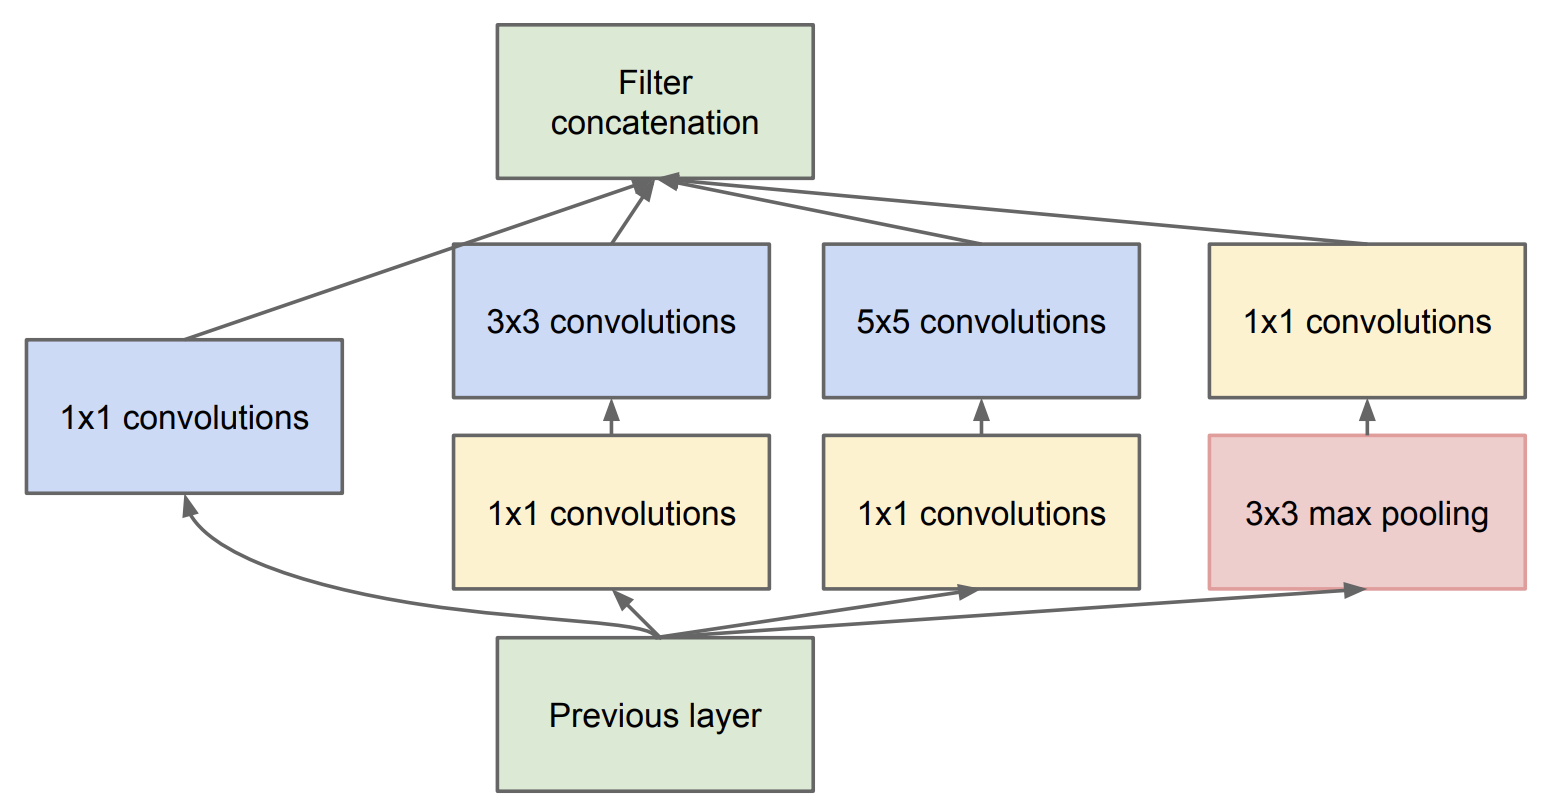
\includegraphics[width=0.95\textwidth]{./figures/inception-module.png}
\end{column}
\begin{column}{0.55\textwidth}
\begin{itemize} \is{2mm}
\item use $1\times 1$ convolutions to \textbblue{reduce dimensionality}
\item adapt dimensionality to size of downstream filter window
\item allows for increasing width (dim reduce) and depth (net-in-net)
\end{itemize}
\end{column}
\end{columns}
\end{frame}

%%%%%%%%%%%%%%%%%%%%%%%%%%%%%%%%%%%%%%%%
\begin{frame} \frametitle{Very deep convolutional networks: VGG}
%%%%%%%%%%%%%%%%%%%%%%%%%%%%%%%%%%%%%%%%
\begin{columns}
\begin{column}{0.48\textwidth}
{\small \textit{Simonyan, Zisserman: Very deep convolutional networks for large-scale image recognition. ICLR 2015 [23k+cit]}}
\end{column}
\begin{column}{0.50\textwidth}
\begin{center}
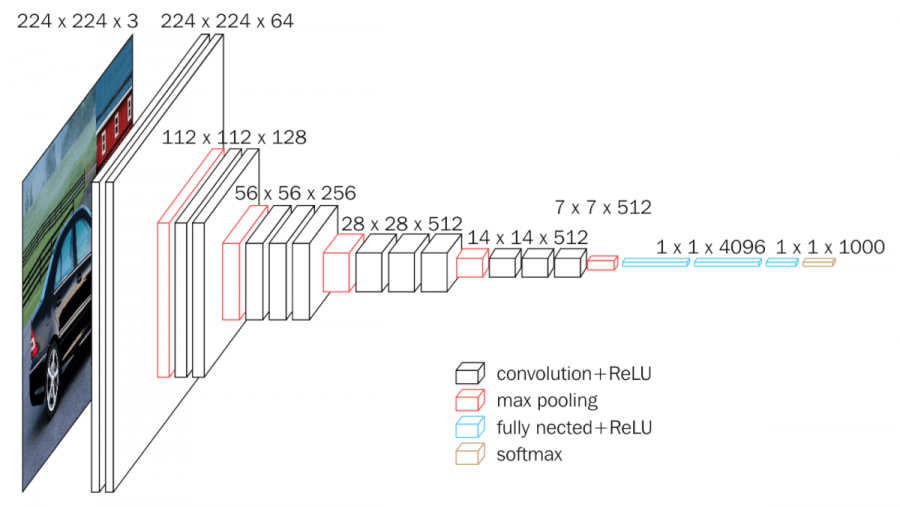
\includegraphics[width=0.99\textwidth]{./figures/vgg.png}
\end{center}
\end{column}
\end{columns}

\begin{itemize} \is{2mm}
\item use very small receptive fields (maximally $3 \times 3$)
\item avoid downsampling/pooling
\item stacking small receptive fields: more depth, fewer parameters
\end{itemize}
\end{frame}



\bibliography{th}
\bibliographystyle{acm}

\end{document}
